\documentclass[letterpaper,12pt]{article}
\usepackage{cite}
\usepackage{graphicx}
\usepackage{amsmath}
\usepackage{adjustbox}
\usepackage{multirow}
\usepackage{caption}
\usepackage{subcaption}
\usepackage{hyperref}
\newcommand{\RN}[1]{%
  \textup{\uppercase\expandafter{\romannumeral#1}}%
}
\captionsetup[figure]{labelsep=period}
\captionsetup[subfigure]{labelformat=simple} % default is 'parens'
\renewcommand\thesubfigure{\thefigure.\alph{subfigure}.}
\DeclareMathOperator*{\argmax}{argmax}
\DeclareMathOperator*{\argmin}{argmin}
\newtheorem{corollary}{CorollaURry}

\begin{document}
    
\title{\bfseries{Query expansion using Language Models}}
\author{Flavio Forenza}
\date\today
\maketitle

\begin{abstract}
  The use of different methods of language modeling, within the field 
  of information retrieval, is finding a wide diffusion in the state of the 
  art. Based on the accuracy of the language model, the problem related 
  to the information retrieval, in a large corpus of documents, can be 
  solved. In order to do this, the basic idea of these approaches is to 
  estimate a probabilistic linguistic model, for each document in the 
  collection, which is able to generate a ranking of relevant documents 
  given a query. One of the problems that afflicts this family of methods 
  is due to the lack of data present. From this, it is necessary to apply 
  smoothing techniques capable of adjusting the maximum likelihood 
  estimator in order to correct the generated imprecision. This paper 
  shows how their application outperforms the performance of classic 
  methods, such as \emph{tf-idf}, useful for generating rankings of 
  documents ordered by relevance. Using them, we will look at some concepts that 
  are useful for query expansion.
\end{abstract}

\section*{Introduction}
Over the years, query expansion techniques have been proposed as a solution 
to the problem of term mismatches between a query and its relevant documents. 
There are typically two types of query expansion method families: 
Local (based on Pseudo / Relevance / Indirect Feedback) and Global (based 
on the generation and use of a thesaurus) \cite{01}. This paper focuses on the 
first category. Given the difficulty in gathering the users' feedback, only the 
first documents recovered will be considered relevant. Pseudo-relevant documents 
are used to find possible candidate terms to help expand the query \cite{02}.
This method has been further developed within the concept of the Language
Model\cite{06}. Statistical language models are widely used within Information 
Retrieval as they have a solid theoretical background and good empirical performance. 
At the state of the art, two well known probabilistic approaches 
in infromation retrieval are the Robertson and Sparck Jones model \cite{07} and 
the Croft and Harper model \cite{08}. Both models estimate the probability of relevance 
of each document to the query. Clearly, the two main problems relate 
to correctly estimating both the query model and the document model. A 
Language Model calculates the relevance of a document \emph{d} to a query \emph{q} by 
estimating a factored form of the distribution $P (q, D)$ \cite{03}. The construction 
of a good Language model must necessarily make use of smoothing models 
when one or more terms do not appear in a document. In the latter case, the 
maximum likelihood estimator would produce a probability equal to zero, 
invalidating the creation of the model itself \cite{04}\cite{05}. Another concept, useful 
for expanding the query and widely used within the project, is that of 
\emph{Word Embeddings}. The latter is obtained precisely from the use of Language 
models, or rather thanks to the co-occurrence of the terms made available. 
This method is based on being able to map every single word into a vector of 
real numbers, within a vector space. The idea is to be able to compare the 
distance of these in order to understand their similarity relationship. If one 
word is similar to another, then these will be considered as synonyms. The 
remainder of the paper is organized as follows. In the next section, \emph{Research 
question and Methodology}, the objectives of the project will be introduced 
followed by an overview of the proposed approach. The third section, \emph{Experimental 
result}, describes the whole system and the results obtained. Finally, 
the conclusions are presented in section four, \emph{Concluding remarks}.

\section*{Research question and Methodology}

Language models can be used for a variety of purposes, such as: speech recognition, 
spelling correction, grammar correction and automatic translation. 
All these applications have the task of assigning a probability to a 
sequence of words, based on the number of times they appear in one or more 
documents. As briefly mentioned in the introductory chapter, the purpose 
of the following project is to verify the existence of a further method, which 
makes use of the concept of language model, specifically an \emph{n-grams} model, 
capable of expanding a query. Achieving this goal means solving the problem 
of mismatch between the terms present in the query and those present in a 
corpus of documents. The probability of generating a new \emph{q} query given the 
estimate of a Language Model for a \emph{D} document can only occur through a 
ranking of relevant documents. If the corpus of documents is large, thinking 
of generating \emph{n} Language models, with \emph{n} equal to the number of documents, 
turns out to be a computationally expensive operation. This paper has used 
a useful approach to be able to generate a first ranking of documents ordered 
by relevance with the query \emph{q}. The technique applied is the \emph{tf-idf} recovery 
model. The adoption of this method of weighing the terms, as well as being 
widely used in the state of the art, produces excellent results. The introduction 
of the \emph{LM}, and of other semantic analysis techniques, made it possible 
to outperform the performance of the \emph{tf-idf} baseline, generating ranking, 
starting from the latter, of documents more pertinent to the query \emph{q} \cite{09}. In 
the following paper, tests are carried out which certify the veracity of this 
thesis. It should be noted that the generation of the ranking, obtained from 
the weights of the \emph{tf-idf} method, is obtained using the well-known \emph{cosine 
similarity} metric between the weight vectors. To comply with the set objective, 
the position of the relevant target document, that is the document 
that the user is searching for, was kept track. This was possible because a 
query was chosen, among those available, that was close to the title of 
this document. The score assigned to the target document will represent the 
minimum \emph{threshold} to be able to form the new ranking of documents. This step 
is fundamental as, by setting a higher threshold, the target document would 
be lost in subsequent calculations. By setting a lower threshold, however, 
those documents that represent noise will be taken into account. From this 
ranking, the \emph{LMs} for each document will be calculated \cite{10}, generating \emph{n} LMs, 
with \emph{n} equal to the number of relevant documents, based on the terms in the 
query. It should be noted that, in order to carry out this step, the concept 
of \emph{skip-gram} has been applied to the query, with step \emph{s} equal to two. The 
creation of each LM is possible only after using one of the existing smoothing 
techniques. To prevent a linguistic model from assigning zero probability to 
an invisible event, i.e. when a term present in the query is not present in 
an LM, we should eliminate some probability mass from some more frequent 
events and give it to events that we haven't never seen. There 
are a variety of methods for smoothing, some of these are: \emph{Laplace (add-
one) smoothing}, \emph{Linear Interpolation smoothing}, \emph{add-k smoothing}, \emph{back-off 
smoothing} and \emph{Kneser-Ney smoothing}. Among these, the following paper 
has experimented the use of the first two smoothing methods, each of which 
will produce different results useful for achieving the final goal. The core of 
the algorithm lies in being able to derive the best ranking of relevant documents, 
using the initial query, through an iterative process, as s changes. 
This variation will lead to the generation of several LMs, each with step \emph{s}, 
with $s=\{2,3,\ldots,10\}$. At each iteration, a new ranking of documents will be generated, thanks to the calculation of the Maximum Likelihood Estimation \emph{MLE}, between the query \emph{q} and each document \emph{d}(\ref{MLE}).
\begin{eqnarray}\label{MLE}
    P(q|d) & \approx & P(q|M_d) \nonumber \\
           & \approx & \prod_i^n{P(w_i|w_{i-1})} \nonumber \\
           & \approx & \frac{count(w_i,w_{i-1})}{\sum_{j=1}^n count(w_j,w_{i-1})} \nonumber \\
           & = & \frac{count(w_i, w_{i-1})}{count(w_{i-1})}
\end{eqnarray}
Among all these nine rankings, after being sorted, the one that will have the 
target document in the highest position, close to the first, will be chosen. 
Also thanks to this, it will be possible to determine the lambda parameters 
present in the interpolation smoothing technique. By focusing on the latter 
technique, it was necessary to implement the concept suggested by \cite{11} as 
regards the calculation of linear interpolation. Instead of adding one to 
the probability calculation, as is well known in Laplace's smoothing (\ref{Laplace}), linear 
interpolation, recursively, calculates the MLE of order two (\emph{bi-grams}) (\ref{LinInt}), up to 
the order zero (\emph{zero-grams})(\ref{zero-grams}).
\begin{equation}\label{Laplace}
    P(w_i|w_{i-1}) = \frac{count(w_{i-1})+1}{count(w_{i-1})+|V|}
\end{equation}
\begin{equation}\label{LinInt}
    P(w_i|w_{i-1}) = \lambda P(q|M_d) + (1-\lambda)P(q|M_c)
\end{equation}
\begin{equation}\label{zero-grams}
    P(w_i) = \lambda \frac{1}{|V|} + (1-\lambda)P(w_i)
\end{equation}

where:
\begin{itemize}
    \item $\sum_i \lambda_i = 1$
    \item $M_d$: represents the language model of the single document;
    \item $M_c$: represents the language model of the entire collection of documents;
    \item $|V|$: represents the number of unique words within the corpus of documents.
\end{itemize}
It is always good to specify that, like the iterative process of steps \emph{s}, both $\lambda$ 
parameters also follow the same reasoning. The idea is to assign a range of 
numbers $\lambda = \{0.1, 0.2,\ldots,1\}$ to both values. In both smoothing techniques, 
the \emph{perplexity} level existing between the query word set $W = \{w_1, w_2,\ldots,w_N\}$ and the language model of 
the target document present in the ranking of relevant documents returned 
by the tf-idf model will be calculated(\ref{perplexity}) \cite{12}.
\begin{equation}\label{perplexity}
    pp(W) = \sqrt[n]{\prod_{i=1}^N\frac{1}{P(w_i|w_{i-1})}} 
\end{equation}
After obtaining the best ranking, the next step is based on building a \emph{term-
term matrix} \cite{12}, where the terms in question are both those of the query and 
those belonging to the language model of the entire collection of relevant 
documents present in the ranking. Within this matrix, the numbers of co-occurrences 
between all terms will be reported. On this type of matrix it is 
possible to apply the calculation of \emph{Positive Pointwise Mutual Information 
(PPMI)}. PPMI draws on the intuition that the best way to weigh the association 
between two words is to ask how much more the two words co-occur in 
our corpus than we would have a priori expected them to appear by chance. 
This measure derives from the calculation of the standard PMI which represents 
a measure of frequency between two events \emph{x} and \emph{y}, compared to what 
we would expect if they were independent (\ref{pmi}).
\begin{equation}\label{pmi}
    \emph{pmi(x,y)} = \log_2\frac{P(x,y)}{P(x)P(y)}
\end{equation}
The ratio gives us an estimate of how much more the two words co-occur 
than we expect by chance. PMI values can be positive, negative or infinite. 
Negative values, which imply that events occur less often than we would 
expect by chance, tend to be unreliable when we have documents consisting 
of few terms, as in our case. To solve this problem, the calculation of the 
PPMI is used which replaces negative values with zero(\ref{ppmi}).
\begin{equation}\label{ppmi}
    PPMI(x,y) = \max(\log_2\frac{P(x,y)}{P(x)P(y)}, 0)
\end{equation}
But the question is: why is the PPMI calculation used? The adoption of 
this is useful for being able to calculate the similarity between words, i.e. 
their synonymy, search for paraphrases, keep track of the change in meaning 
of words and to automatically discover the meanings of words in different 
corpora. To find the words most similar to those in the query, the cosine 
similarity is calculated on the first ten word vectors that have the highest 
positive PPMI values. Eventually, each token in the query will have a maximum 
of ten expansion terms. Thanks to this, we are already seeing how 
query expansion can be done. Moving on, there is a problem to solve before we can 
calculate the similarity of the cosine: the \emph{sparsity} of the matrix. In order to 
obtain a good similarity, relatively low at the computational level, another 
concept has been implemented: \emph{Singular Value Decomposition (SVD)}. The 
idea of applying SVD on a term-term matrix was proposed by \cite{13}. Switching 
from sparse to dense vectors allows for better similarity comparisons. The 
SVD allows to decompose the term-term matrix (A), of dimensions $txd$, into 
three matrices \cite{14} (\ref{decomposition}):
\begin{equation}\label{decomposition}
    A = USV^t
\end{equation}
Where:
\begin{enumerate}
    \item \emph{U}: matrix of dimension $txm$ where the columns represent the left 
    singular vectors of matrix A;
    \item \emph{S}: diagonal matrix of dimension $mxm$, containing the singular values 
    of matrix A;
    \item \emph{$V^T$}: transposed matrix, of dimensions $mxd$, where the columns represent 
    the right singular vectors of matrix A.
\end{enumerate}
Thanks to the product of the matrix \emph{U} with the matrix \emph{S}, a new matrix 
\emph{$\mathcal{D}$} (\ref{matrixD}), of dimension $txm$, is formed containing all the terms that will be 
compared, through cosine similarity, with the query terms present in the 
matrix \emph{$\mathcal{T}$} (\ref{matrixT}) given by the product of \emph{S} and $V^T$ .
\begin{equation}\label{matrixD}
    \mathcal{D} = U*S
\end{equation}
\begin{equation}\label{matrixT}
    \mathcal{T} = S*V^T
\end{equation}
Having all the possible words available to be added to the query tokens, the 
time has come to generate all the possible queries. The number of queries 
produced will depend on the number of words present in the initial query and 
on any words obtained from the calculation of the cosine similarity. Having 
set a maximum limit of ten words per token, the total of the quries generated 
is given by the product (\ref{possQueries}) of the number of possible pairs of terms: 
\begin{equation}\label{possQueries}
    \#Queries = \prod_i^N \#new\_tokens_i
\end{equation}
where \emph{i} is the i-th token of the query and N is the len of the query. Being new 
queries, these will be subjected to the same procedure as the original query, 
that is, new LMs will be produced and with them new rankings of documents 
that will contain the target document in the first positions. Finally, the best 
query, or queries, will be chosen based on the level of perplexity reached.

\section*{Experimental Results}

The dataset used for the experiments is the famous \emph{Recipes1M+} \cite{15}, a collection 
created by MIT, consisting of more than one million culinary recipes. 
Of all these recipes, only a subset of 51235 documents of it was used due 
to their informative content which best fits the purpose of this study. The 
information about the line distributions for each recipe indicates that the 
instruction field contains a higher number than the information contained in 
the ingredients field. To have good performance in finding, we preferred to 
choose the "instructions" field (\ref{distributions}). The first ranking of relevant documents, 
generated by the tf-idf method, was evaluated following two different 
approaches that could best be linked with the principle explained in \cite{16}. 
Specifically, each category of a recipe is considered as an entity associated 
with a document. Both approaches rely on being able to compare the categories of relevant documents 
with the category of the target document. Since the categories are not present in the dataset, the 
two proposed approaches deal with being able to "extract" these categories directly from the web. 
\begin{figure}[h!]
    \centering
    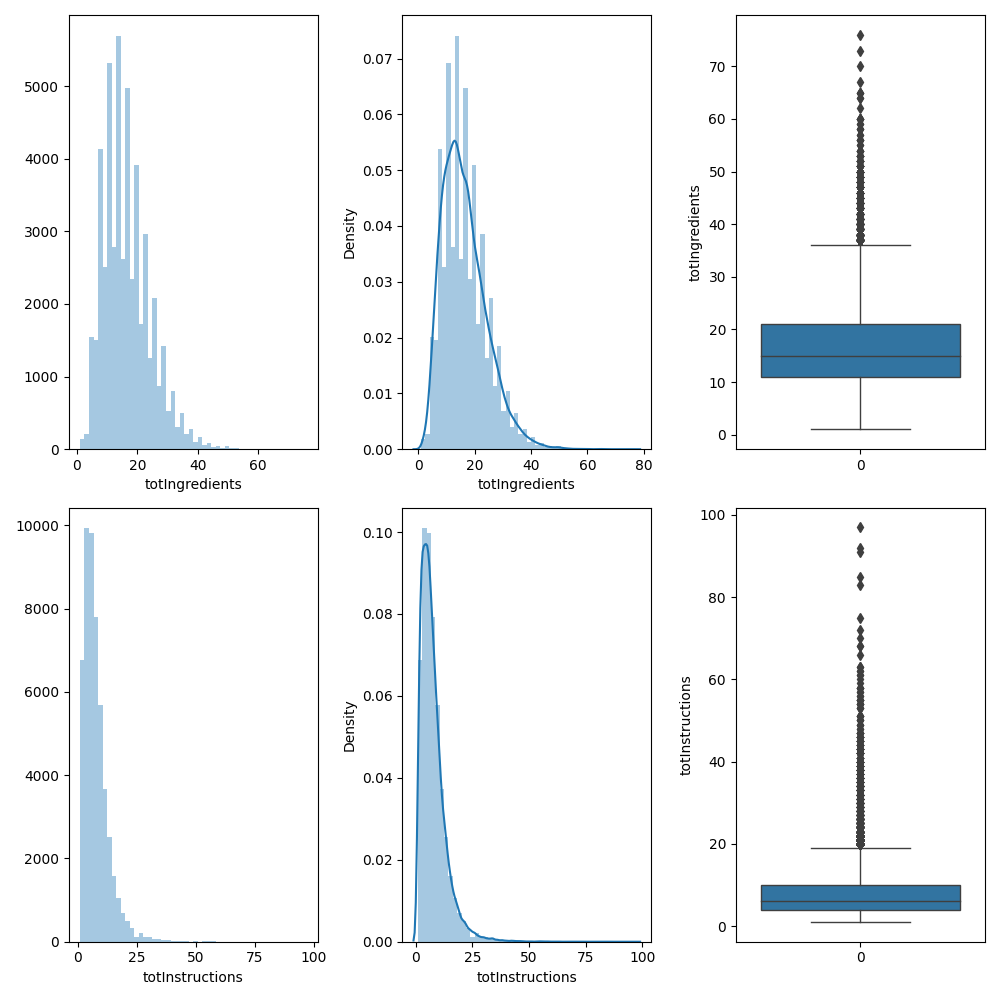
\includegraphics[width = 0.7 \linewidth]{images/displot.png}
    \centering
    \caption{Dstributions of lines per ingredients and instructions.}
    \label{distributions}
\end{figure}
The first approach uses an API, called \href{https://pypi.org/project/scrape-schema-recipe/}{\emph{Scrape Schema Recipe}}, 
which takes the link associated with the recipe website, present in the dataset, and scrapes the corresponding category.
Unfortunately not all the links are still existing, therefore the evaluation of the ranking takes place following three types of methods:
\begin{enumerate}
    \item {\bfseries Overestimated}: consider the uncategorized document as good;
    \item {\bfseries Underestimated}: considers the uncategorized document not good;
    \item {\bfseries Discarded}: Discard the uncategorized document from the evaluation.
\end{enumerate}
As for the second method, this makes use of the \href{https://fdc.nal.usda.gov/api-guide.html}{\emph{USDA}} API, a library that has the task 
of taking every single ingredient of the recipe and fetching the corresponding category from a large database belonging to the United States 
Department of Agriculture. Compared to the first approach, the recipes that did not have a category are only four recipes. It is worth mentioning 
that both approaches are computationally expensive as the extraction of all categories took about two days. In addition to all these evaluations, 
it was decided to create a last one derived from a mixed approach (Scrape + USDA). Taking five random queries, the evaluations of the corresponding 
rankings are those reported in table (\ref{avgp}).
\begin{table}[h!]
    \centering
    \begin{adjustbox}{max width=\textwidth}
    \begin{tabular}{|c||c|c|c||c||c||}
        \hline
        \multirow{2}{*}{\bfseries{Queries}} & \multicolumn{3}{c||}{\bfseries{Scrape Schema Recipe}} & \multicolumn{1}{c||}{\bfseries{USDA}} & \multicolumn{1}{c||}{\bfseries{Mixed (Scrape+USDA)}} \\            & \bfseries{Overestimate} & \bfseries{Underestimate} & \bfseries{Discarded} & \bfseries{}  & \bfseries{}\\
        \hline
        \hline
        \RN{1} & 0.7520 & 0.3734 & 0.5958 & 0.9817 & 0.9947\\
        \hline
        \RN{2} & 0.9309 & 0.6780 & 0.9054 & 1.0 & 1.0\\
        \hline 
        \RN{3} & 0.7458 & 0.2746 & 0.5411 & 0.9797 & 0.9982\\
        \hline
        \RN{4} & 1.0 & 0.6401 & 1.0 & 1.0 & 1.0\\
        \hline
        \RN{5} & 0.9098 & 0.4885 & 0.8456 & 0.9934 & 0.9934\\
        \hline
        \hline
        Average & 0.8677 & 0.4909 & 0.77758 & 0.99096 &  \bfseries 0.99726 \\
        \hline
    \end{tabular}
    \end{adjustbox}
    \caption{Average Precision on each query for each method.}
    \label{avgp}
\end{table}
As you can see, the mixed approach is the one that, in terms of average precision, manages to achieve the best evaluation.
Moving on to the evaluation of the new queries generated, a visual comparison, based on a PCA, was used between the ranking generated by the tf-idf method and each new query produced by the project core. The goal is to find a query whose distance from the target document is less than all other distances produced by the remaining queries.

\newpage
\bibliographystyle{abbrv}
\bibliography{Bibliography}

\end{document}